\section{Test af det endelige system}
\label{TestAfDetSamledeSystem}


\begin{table}[H]
\centering
\begin{tabular}{|l|l|l|l|l|l|}
\hline
V & 0.90 & 1.30 & 1.90 & 2.40 & 2.90 \\ \hline
THD \% & 4.26 & 0.29 & 0.09 & 0.05 & 0.14 \\ \hline
\end{tabular}
\caption{Den målte THD af det endelige system uden filtre}
\label{tab:THDEndeligeSystem}
\end{table}
THD for det endelige system holder sig indenfor det acceptable. Bortset fra når volumenkontrollen er skruet helt i bund, her er THD'en på $4.26\%$ hvilket er lidt over kravet. At THD overskrider kravet når volumen er skruet helt ned for volumen gør at det ikke vurderes katastrofalt.
%

\begin{figure}[H]
	\centering
	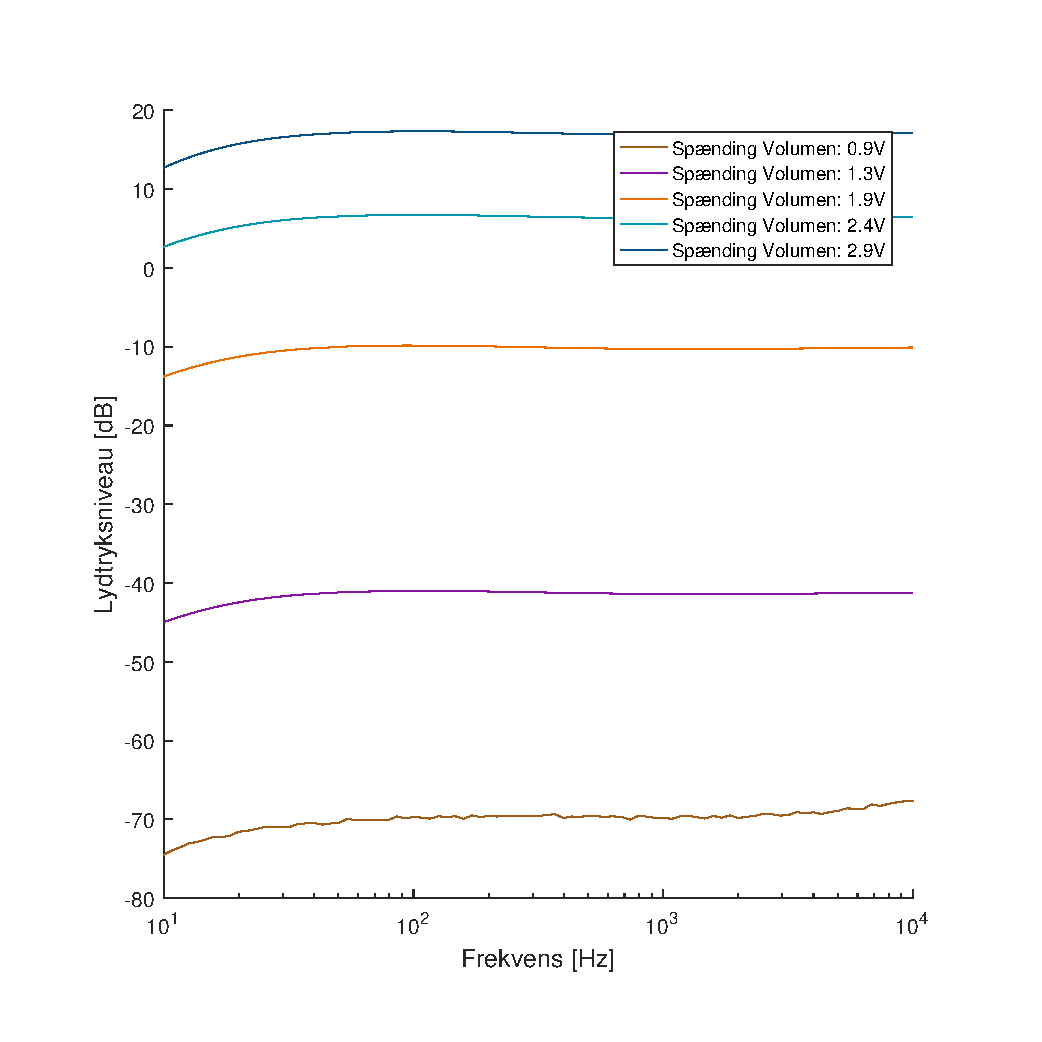
\includegraphics[resolution=300,width=\textwidth]{Figure/FrekvensResponsEndeligeSystemUdenFiltre.pdf}
	\caption{Frekvensrespons for det samlede system hvor der ikke er valgt nogle filtre}
	\label{fig:FrekvensResponsEndeligeSystemUdenFiltre}
\end{figure}
\noindent
%
Frekvensresponsen er ideelt flad ved alle lydtryksniveauer, og det er den tildels også, med små udsving omkring de lave frekvenser. Dette når dog at rette sig ud inden 20Hz så afvigelserne ikke vurderes katastrofale.

Der var auditive kliklyde ved skift af filter, både med og uden lydsignal på indgangen. Dette menes at være forårsaget af et DC-offset imellem filtrene. Der blev ikke målt videre på dette, men det skønnes, at en AC-kobling på udgangene af hvert filter skulle kunne afhjælpe denne effekt.
%Samlet black-box test af hele systemet